% !TEX program = xelatex
% 使用 texlive完整编译:
% xelatex -> bibtex -> xelatex -> xelatex
% SHNU-Thesis 上海师范大学研究生 LaTeX 模板
\documentclass{shnuthesis}
% 进行个人信息设置
\title{这是一个很长的这是一个很长的这是一个很长的毕业论文题目}
\author{某~~某~~某}           % 作者姓名
\date{2\,0\,2\,1~~年~~3~~月}  % 完成日期
\college{学~~院~~名~~称}
\major{专~~业~~名~~称}  % 专业名称
\study{专~~业~~方~~向~~名~~称}
\stunum{123000678}     % 学号
\classifnum{O24}       % 分类号
% 中图分类号 计算数学 O24; 基础数学 O15; 应用数学 O29
\instructor{某~~某~~某~~~~教~~授}  % 导师姓名

% 添加自己要用的其他宏包
\usepackage[numbers]{natbib}
\usepackage{subfig}
% \usepackage{xltxtra}

% --- 证明结束黑框 ----
% \renewcommand{\qedsymbol}{$\blacksquare$}

% --- 设置英文字体 -----
\usepackage{newtxtext}  % for text fonts

% --- 设置数学字体 -----
% \usepackage{newtxmath}
% \usepackage{mathptmx}

% --- 直接插入 pdf 文件 ----
% \usepackage{pdfpages}

% --- 自定义命令 -----
\newcommand{\CC}{\ensuremath{\mathbb{C}}}
\newcommand{\RR}{\ensuremath{\mathbb{R}}}
\newcommand{\A}{\mathcal{A}}
\newcommand{\ii}{\bm{\mathrm{i}}\,}  % 虚部
\newcommand{\md}{\mathrm{d}\,}
\newcommand{\bA}{\boldsymbol{A}}
\newcommand{\red}[1]{\textcolor{red}{#1}}

\begin{document}

\frontmatter

% 生成标题页
\maketitle

% \thispagestyle{empty}
% 需要 pdfpages 宏包
% \includepdf[pages=-]{pdfname.pdf}

% 生成声明与授权书页, 此页可以放在最后
\makestatement


\clearpage   % 结束上一页
\pagenumbering{Roman} % 摘要页码为大写罗马数字


%%%%%%%%%%%%%%%%%%%%% 填写中文摘要内容和关键字  %%%%%%%%%%%%%%%%%%%%%%%%%%%

\begin{cnabstract}{关键词 1;关键词 2;关键词 3}

在正文中添加空行可以实现换行功能.
		
摘要内容摘要内容摘要内容摘要内容摘要内容摘要内容摘要内容摘要内容摘要内容摘要内容摘要内容摘要内容摘要内容摘要内容摘要内容摘要内容摘要内容摘要内容摘要内容摘要内容摘要内容摘要内容摘要内容摘要内容摘要内容.
		
摘要内容摘要内容摘要内容摘要内容摘要内容摘要内容摘要内容摘要内容摘要内容摘要内容摘要内容摘要内容摘要内容摘要内容摘要内容摘要内容摘要内容摘要内容摘要内容摘要内容摘要内容摘要内容摘要内容摘要内容摘要内容.

摘要内容摘要内容摘要内容摘要内容摘要内容摘要内容摘要内容摘要内容摘要内容摘要内容摘要内容摘要内容摘要内容摘要内容摘要内容摘要内容摘要内容摘要内容摘要内容摘要内容摘要内容摘要内容摘要内容摘要内容摘要内容.


\end{cnabstract}


% 填写英文摘要内容和关键字

\begin{enabstract}{Keyword 1;~ Keyword 2;~ Keyword 3}

This is abstract. This is abstract. This is abstract. This is abstract. This is abstract. This is abstract. This is abstract. This is abstract. This is abstract. This is abstract. This is abstract. This is abstract.
		
The quick brown fox jumps over the lazy dog. The quick brown fox jumps over the lazy dog. The quick brown fox jumps over the lazy dog. The quick brown fox jumps over the lazy dog. The quick brown fox jumps over the lazy dog.

The quick brown fox jumps over the lazy dog. The quick brown fox jumps over the lazy dog. The quick brown fox jumps over the lazy dog. The quick brown fox jumps over the lazy dog. The quick brown fox jumps over the lazy dog.


\end{enabstract}
	
    % 生成目录(自定义的命令)
    % 使用方法: \maketoc[nopagenum/pagenum/pagenumtoc]
    % 其中: nopagenum指目录没有页码(默认值);pagenum指目录有页码;
    % pagenumtoc指目录有页码, 且目录两字出现在目录中
    % 请注意在合适的位置放置\pagenumbering{numstyle}使用新的页码
    \maketoc[pagenumtoc]


	\cleardoublepage  % 结束上一页
	\pagenumbering{arabic}  % 正文页码为阿拉伯数字

    \mainmatter

%%%%%%%%%%%%%%%%%%%%%%%%%%%%%% 正文内容从这里开始  %%%%%%%%%%%%%%%%%%%%%%%%%%%%%


\chapter{引言}

\section{研究背景}
这是小四号的正文字体, 行间距 1.35 倍.
	
通过空一行实现段落换行, 仅仅是回车并不会产生新的段落.

自定义了一个命令 \verb|\red{文字}| 可以\red{加红文字}, 可以在论文修改阶段方便标记.

这是一个引用的示例 \cite{Adams2003}和 \cite{Shen1994,Tadmor2012,TreWei2014}.

这是一大段文字这是一大段文字中英文混排 Numerical Methods. 这是一大段文字这是一大段文字这是一大段文字这是一大段文字这是一大段文字这是一大段文字这是一大段文字这是一大段文字这是一大段文字这是一大段文字这是一大段文字这是一大段文字这是一大段文字这是一大段文字这是一大段文字这是一大段文字这是一大段文字这是一大段文字这是一大段文字.

\section{主要结论}

这是一大段文字这是一大段文字这是一大段文字这是一大段文字这是一大段文字这是一大段文字这是一大段文字这是一大段文字这是一大段文字这是一大段文字这是一大段文字这是一大段文字这是一大段文字这是一大段文字这是一大段文字这是一大段文字这是一大段文字这是一大段文字这是一大段文字这是一大段文字这是一大段文字这是一大段文字这是一大段文字这是一大段文字这是一大段文字这是一大段文字这是一大段文字.



\section{结构安排}

本文接下来的写作安排如下:

第二章, 首先介绍了数学公式的使用, 然后介绍了定理环境, 给出了定义、定理、命题、引理、推论、证明以及注的环境示例.

第三章, 对于差分方法数值求解微分方程, 给出了一个简短的示例.

第四章, 针对表格环境, 给出了三线表的介绍和自定义表格环境 generaltab 的使用, 也给出了其他表格插入示例.

第五章, 针对插图环境, 给出了自定义插图环境 generalfig 和 并排插图实例.

第六章, 给出了列表的示例与参考文献样式的设置.

最后是插入参考文献、致谢、攻读硕士学位期间的研究成果和附录环境.



%%%%%%%%%%%%%%%%%%%%%%%%%%%%%% 数学公式与定理  %%%%%%%%%%%%%%%%%%%%%%%%%%%%%%%%

\chapter{数学公式与定理}

\section{数学公式}

数学公式的使用请参考公式手册 symbols-a4, 或者 《一份(不太)简短的 \LaTeX~2$\varepsilon$ 介绍》 (lshort-zh-cn).

自定义命令表示的几个数学符号 $\RR$, $\CC$, $\A$, $\ii$, $\md$, $\bA$.

在文中行内公式可以这么写: $a^2+b^2=c^2$, 这是勾股定理, 它还可以表示为 $c=\sqrt{a^2+b^2}$, 还可以让公式单独一段并且加上编号
\begin{equation}\label{eqn:trifun}
\sin^2{\theta}+\cos^2{\theta}=1.
\end{equation}
还可以通过添加标签在正文中引用公式, 如等式~\eqref{eqn:trifun} 或者 \ref{eqn:trifun}.

读者可能阅读过其它手册或者资料, 知道 LaTeX 提供了 eqnarray 环境. 它按照等号左边—等号—等号右边呈三列对齐, 但等号周围的空隙过大, 加上公式编号等一些 bug, 目前已不推荐使用. (摘自 lshort-zh-cn)

多行公式常用 align 环境, 公式通过 \verb|&| 对齐. 分隔符通常放在等号左边:
\begin{align}
a & = b + c \\
& = d + e.
\end{align}

align 环境会给每行公式都编号. 我们仍然可以用 \verb|\notag| 或 \verb|\nonumber| 去掉某行的编号. 在以下的例子,
为了对齐等号, 我们将分隔符放在右侧, 并且此时需要在等号后添加一对括号 \verb|{}| 以产生正常的间距:
\begin{align}
a ={} & b + c \\
={} & d + e + f + g + h + i + j \notag \\
& + m + n + o \\
={} & p + q + r + s.
\end{align}

如果我们不需要按等号对齐, 只需罗列数个公式, gather 将是一个很好用的环境:
\begin{gather}
a = b + c \\
d = e + f + g \\
h + i = j + k \notag \\
l + m = n
\end{gather}

align 和 gather 有对应的不带编号的版本 align* 和 gather*.

对于 align、 gather、align* 与 gather* 等环境, 在添加命令 \verb|\allowdisplaybreaks| 后 (已添加), 公式可以跨页显示.

多个公式组在一起公用一个编号, 编号位于公式的居中位置, amsmath 宏包提供了诸如 aligned、gathered 等环境, 与 equation 环境套用.

这个公式使用 aligned 环境 (\textbf{推荐使用})
\begin{equation}\label{eqn:1}
\left\{\begin{aligned}
  &-\frac{\mathrm{d}^{2} u}{\mathrm{d} x^{2}}+\frac{\mathrm{d} u}{\mathrm{d} x}=\pi^{2} \sin (\pi x)+\pi \cos (\pi x),\quad x \in [0,1], \\
  &u(0)=0,\quad u(1)=0.
\end{aligned} \right.
\end{equation}

这个公式使用 array 环境
\begin{equation}\label{eqn:2}
\left\{\begin{array}{l}
\displaystyle
-\frac{\mathrm{d}^{2} u}{\mathrm{d} x^{2}}+\frac{\mathrm{d} u}{\mathrm{d} x}=\pi^{2} \sin (\pi x)+\pi \cos (\pi x),\quad x \in [0,1], \\[6pt]
u(0)=0,\quad u(1)=0.
\end{array} \right.
\end{equation}

aligned 与 equation 环境套用, 公式间距是自动调节的, 如果有分式, 分式也是行间显示. 如果用 array 与 equation 环境套用, 有时候需要手动调整公式行间距和行间显示.


\section{定理环境}

\begin{definition}
这是一个定义.
\end{definition}

\begin{lemma}[Lemma] \label{lemma1}
这是一个引理.
\end{lemma}

\begin{theorem}[Theorem]
这是一个定理.
\end{theorem}
\begin{proof}
这是证明环境.
\end{proof}

\begin{proposition}[Proposition]
这是一个命题.
\end{proposition}

\begin{lemma}\label{lemma-convergence} {\rm (\textit{参考文献}\cite{LiLiu1997})}
假设单步法具有 $p$ 阶精度, 且増量函数 $\varphi(x_{n}, u_{n}, h)$ 关于 $u$ 满足 {\rm Lipschitz} 条件
\begin{equation}\label{eqn:3}
|\varphi(x, u, h)-\varphi(x, \bar{u}, h)| \leqslant L_{\varphi}|u-\bar{u}|.
\end{equation}
\end{lemma}

\begin{theorem}\label{theorem-convergence}
假设单步法具有 $p$ 阶精度, 且増量函数 $\varphi(x_{n}, u_{n}, h)$ 关于 $u$ 满足 {\rm Lipschitz} 条件
\begin{equation}\label{eqn:4}
|\varphi(x, u, h)-\varphi(x, \bar{u}, h)| \leqslant L_{\varphi}|u-\bar{u}|.
\end{equation}
\end{theorem}
\begin{proof}
由定理 \ref{lemma1} 和 \eqref{eqn:1} 式可以推出以上结论.
\end{proof}

\begin{corollary}\label{col-convergence}
假设单步法具有 $p$ 阶精度, 且増量函数 $\varphi(x_{n}, u_{n}, h)$ 关于 $u$ 满足 {\rm Lipschitz} 条件
\begin{equation}\label{eqn:5}
|\varphi(x, u, h)-\varphi(x, \bar{u}, h)| \leqslant L_{\varphi}|u-\bar{u}|.
\end{equation}
\end{corollary}


\begin{remark}\label{remark1}
这是一个 remark.
\end{remark}

\begin{example}
这是一个例子.
\end{example}


%%%%%%%%%%%%%%%%%%%%%%%%%%%% 微分方程的数值方法  %%%%%%%%%%%%%%%%%%%%%%%

\chapter{微分方程的数值方法}

本章我们考虑具有以下微分方程:
\begin{equation}\label{eqn:pde}
\left\{\begin{aligned}
& L u=-\frac{\mathrm{d}^{2} u}{\mathrm{d} x^{2}}+\frac{\mathrm{d} u}{\mathrm{d} x}+q u=f, \quad a < x < b, \\
& u(a)=\alpha, \quad u(b)=\beta.
\end{aligned}\right.
\end{equation}
其中 $q, f$ 为 $[a,b]$ 上的连续函数, $q \geqslant 0$; $\alpha, \beta$ 为给定常数. 这是最简单的椭圆方程第一边值问题 .

问题 \eqref{eqn:pde} 存在唯一解 (引用示例参考文献 \cite{LiLiu1997}).


\section{有限差分方法}
在偏微分方程的数值解法中, 有限差分法数学概念直观, 推导自然, 是发展较早且比较成熟的数值方法. 由于计算机只能存储有限个数据和做有限次运算, 所以任何一种用计算机解题的方法, 都必须把连续问题 (微分方程的边值问題、初值问题等) 离散化, 最终化成有限形式的线性代数方程组.

\subsection{数值格式}
将区间 $[a,b]$ 分成 $N$ 等分, 分点为
\begin{equation*}
  x_{i}=a+i h \quad i=0,1, \cdots, N,
\end{equation*}
其中 $h=(b-a) / N$. 于是我们得到区间 $I=[a,b]$ 的一个网格剖分. $x_i$ 称为网格的节点, $h$ 称为步长.

数值格式:
\begin{equation*}
  L_{h} u_{i}=-\frac{u_{i+1}-2 u_{i}+u_{i-1}}{h^{2}}+\frac{u_{i+1}-u_{i-1}}{h}+q_{i} u_{i}=f_{i},\quad 1 \leqslant j \leqslant N-1.
\end{equation*}
其中  $q_{i}=q(x_{i}), f_{i}=f(x_{i})$.

以上差分方程对于 $i=1,2, \cdots, N-1$ 都成立, 加上边值条件 $u_{0}=\alpha, u_{N}=\beta$, 就得到关于 $u_i$ 的差分格式:
\begin{equation}\label{eqn:fdm}
\left\{\begin{aligned}
& L_{h} u_{i}=-\frac{u_{i+1}-2 u_{i}+u_{i-1}}{h^{2}}+\frac{u_{i+1}-u_{i-1}}{2h}+q_{i} u_{i}=f_{i}, \quad i=1,2, \cdots, N-1, \\
& u_{0}=\alpha, \quad u_{N}=\beta.
\end{aligned}\right.
\end{equation}

它的解 $u_i$ 是 $u(x)$ 在 $x=x_i$ 处的差分解.


\subsection{矩阵形式}

先定义向量 $\boldsymbol{u}$:
\begin{equation*}
  \boldsymbol{u}=(u_{1}, u_{2}, \cdots, u_{N-1})^{\mathrm{T}}.
\end{equation*}

差分格式可以写为矩阵形式:
\begin{equation*}
  \boldsymbol{A}\boldsymbol{u}=\boldsymbol{f}.
\end{equation*}
其中矩阵 $\boldsymbol{A}$、向量 $\boldsymbol{f}$ 的定义如下, 注意向量 $\boldsymbol{f}$ 的首尾元素已包含了 $x=a$ 和 $x=b$ 处的边界条件.
\begin{equation}\label{equ:matrix1}
\boldsymbol{A}=\begin{bmatrix}
\dfrac{2}{h^{2}}+q_{1} & \dfrac{1}{2h}-\dfrac{1}{h^{2}} &   &  &  \\[8pt]
 -\dfrac{1}{2h}-\dfrac{1}{h^{2}} & \dfrac{2}{h^{2}}+q_{2} & \dfrac{1}{2h}-\dfrac{1}{h^{2}}  & &  \\[8pt]
  &  &  &  &    \\
   &  \ddots  & \ddots  &  \ddots  &  \\[8pt]
   &  &  &  &    \\
  &   & -\dfrac{1}{2h}-\dfrac{1}{h^{2}} & \dfrac{2}{h^{2}}+q_{N-2}& \dfrac{1}{2h}-\dfrac{1}{h^{2}} \\[8pt]
  &  &  & -\dfrac{1}{2h}-\dfrac{1}{h^{2}} & \dfrac{2}{h^{2}}+q_{N-1}
\end{bmatrix}.
\end{equation}

上一个矩阵用了 \verb|bmatrix| 环境, 也可以使用 \verb|array| 环境.
\begin{equation}\label{equ:matrix2}
\boldsymbol{A}=\left[\begin{array}{cccccc}
\dfrac{2}{h^{2}}+q_{1} & \dfrac{1}{2h}-\dfrac{1}{h^{2}} &   &  &  \\[8pt]
 -\dfrac{1}{2h}-\dfrac{1}{h^{2}} & \dfrac{2}{h^{2}}+q_{2} & \dfrac{1}{2h}-\dfrac{1}{h^{2}}  & &  \\[8pt]
  &  &  &  &    \\
   &  \ddots  & \ddots  &  \ddots  &  \\[8pt]
   &  &  &  &    \\
  &   & -\dfrac{1}{2h}-\dfrac{1}{h^{2}} & \dfrac{2}{h^{2}}+q_{N-2}& \dfrac{1}{2h}-\dfrac{1}{h^{2}} \\[8pt]
  &  &  & -\dfrac{1}{2h}-\dfrac{1}{h^{2}} & \dfrac{2}{h^{2}}+q_{N-1}
\end{array}\right].
\end{equation}



%%%%%%%%%%%%%%%%%%%%%%%%%%%%%% 表格环境  %%%%%%%%%%%%%%%%%%%%%%%%%%%%%%%%%%%%%%

\chapter{表格环境}

\section{表的使用}

作为论文, 推荐使用三线表进行排版. 所谓三线表, 即在标题前有横线, 标题后有横线, 表格最后还有横线, 其他地方无线. 当然这不是死规定, 也可以根据需要在合适的地方加线.

本文定义了新的可变长度左中右 (LCR) 格式, LCR 三个格式会根据表格宽度的设定自行控制宽度, 且其宽度相等, 方便设置和页面相同宽度的表格. 本文还定义了 \verb|P{}| 格式可以设定某一列宽度 (如 \verb|P{1cm}| 控制某一列的宽度为 1cm), \verb|P{}| 格式在 \verb|p{}| 格式的基础上增加了居中功能. PLCR 格式的功能需要使用 tabularx 做表.

\section{表格示例}

可以使用自定义表格环境 generaltab.

\begin{generaltab}{某校学生升高体重样本.}{tab:heightweight}
		\begin{tabularx}{0.9\textwidth}{lCCC}
			\toprule
			序号&年龄&身高&体重\\
			\midrule
			1&14&156&42\\
			2&16&158&45\\
			3&14&162&48\\
			4&15&163&50\\
			\cmidrule{2-4}
			平均&15&159.75&46.25\\
			\bottomrule
		\end{tabularx}
\end{generaltab}

使用通用的表格环境 table.

\begin{table}[!htp]
\centering
% PLCR已经定义
\caption{某校学生升高体重样本.}
\label{tab2:heightweight}
\begin{tabularx}{0.9\textwidth}{lCCC}
   \toprule
	序号&年龄&身高&体重\\
	\midrule
	1&14&156&42\\
	2&16&158&45\\
	3&14&162&48\\
	4&15&163&50\\
    \cmidrule{2-4}
	平均&15&159.75&46.25\\
	\bottomrule
\end{tabularx}
\end{table}


通过 \verb|ref| 引用表格: 表 \ref{tab2:heightweight}.

通过 \verb|autoref| 引用表格: \autoref{tab2:heightweight}.


\clearpage
基于 tabular 设置一些格式: 上下表格线加粗

\begin{table}[!htp]
%\small
\centering
\caption{数值误差与收敛速率示例.}
\renewcommand\arraystretch{1.2} %定义表格高度
\label{table1}
\begin{tabular}{c|c|cc|cc|cc}
\Xhline{2\arrayrulewidth}
degree &  step-size~$h$  & $L^2$-errors  &  order  & $H^1$-errors & order & $L^\infty$-errors  &  order \\
\hline
   &  1/128    & 9.18E-06    &2.02    & 7.70E-03  &1.01       & 6.46E-07    &2.02    \\
1  &  1/256    & 2.29E-06    &2.01    & 1.92E-03  &1.00       & 1.61E-07    &2.01      \\
   &  1/512    & 5.70E-07    &2.00    & 9.56E-04  &1.00       & 4.01E-08    &2.00       \\
\hline  %   \cline{1-8}
   &  1/128    & 1.39E-08    &3.01    & 1.15E-05  &2.01       & 3.48E-12   &4.02       \\
2  &  1/256    & 1.73E-09    &3.01    & 2.88E-06  &2.01       & 3.27E-13   &3.94      \\
   &  1/512    & 2.17E-10    &3.00    & 7.24E-06  &2.00       & 6.66E-13   &1.55     \\
\hline  %   \cline{1-8}
   &  1/32     & 2.28E-09    &4.05    & 6.92E-07  &3.04       & 1.45E-15   &8.21       \\
3  &  1/64     & 1.42E-10    &4.03    & 8.65E-08  &3.02       & 2.06E-14   &3.85       \\
   &  1/128    & 8.91E-12    &4.01    & 1.08E-08  &3.01       & 3.86E-14   &0.91       \\
\Xhline{2\arrayrulewidth}
\end{tabular}
\end{table}

基于 tabular 设置一些格式: 左右表格双线

\begin{table}[htp!]
\centering
\renewcommand\arraystretch{1.2} %定义表格高度
% PLCR已经定义
\caption{数值误差示例.}
\label{table2}
\begin{tabularx}{0.9\textwidth}{||P{1cm}|C|C|C|C|C|C||}
\Xhline{2\arrayrulewidth}
N  & A       & B    & C       & D      & E       & F   \\
\Xhline{2\arrayrulewidth}
2  & 9.20E-05 & 9.90E-05 & 1.00E-06 & 8.00E-06 & 1.50E-05 & 6.70E-05 \\
4  & 9.80E-05 & 8.00E-05 & 7.00E-06 & 1.40E-05 & 1.60E-05 & 7.30E-05 \\
6  & 4.00E-06 & 8.10E-05 & 8.80E-05 & 2.00E-05 & 2.20E-05 & 5.40E-05 \\
8  & 8.50E-05 & 8.70E-05 & 1.90E-05 & 2.10E-05 & 3.00E-06 & 6.00E-05 \\
10 & 8.60E-05 & 9.30E-05 & 2.50E-05 & 2.00E-06 & 9.00E-06 & 6.10E-05 \\
12 & 1.70E-05 & 2.40E-05 & 7.60E-05 & 8.30E-05 & 9.00E-05 & 4.20E-05 \\
14 & 2.30E-05 & 5.00E-06 & 8.20E-05 & 8.90E-05 & 9.10E-05 & 4.80E-05 \\
16 & 7.90E-05 & 6.00E-06 & 1.30E-05 & 9.50E-05 & 9.70E-05 & 2.90E-05 \\
18 & 1.00E-05 & 1.20E-05 & 9.40E-05 & 9.60E-05 & 7.80E-05 & 3.50E-05 \\
20 & 1.10E-05 & 1.80E-05 & 1.10E-04   & 7.70E-05 & 8.40E-05 & 3.60E-05  \\
\Xhline{2\arrayrulewidth}
\end{tabularx}
\end{table}

	
%%%%%%%%%%%%%%%%%%%%%%%%%%%%% 插图环境  %%%%%%%%%%%%%%%%%%%%%%%%%%%%%%%%

\chapter{插图环境}

\section{图的使用}

XeLaTeX 环境下可以使用 EPS、PDF、PNG、JPEG、BMP 格式的图片, 当然也可以用绘图包直接在 \LaTeX 中绘制图形, 推荐使用宏包 tikz. 图的环境是 figure, 但 figure 环境使用复杂且不自带标题, 因此本模板定义了一个通用版本的 generalfig, 该环境会将 figure 内的图片居中并设置标签与引用名, 同时会让图片位置设置为所有可行位置 (htbp, 即此处、页顶、页底、独立一页), 此选项可以作为可选参数设置.

\section{插图示例}

使用自定义环境 generalfig.

\begin{generalfig}[htb]{大数据信息处理框架.}{fig:data}
		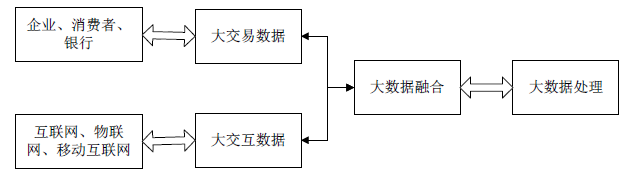
\includegraphics[width=0.9\linewidth]{data.png}
\end{generalfig}

请注意 generalfig 第一个参数是标题, 第二个参数是引用的 label.

两个图左右并排放置, 共用一个标题.
\begin{figure}[htp!]
\centering
  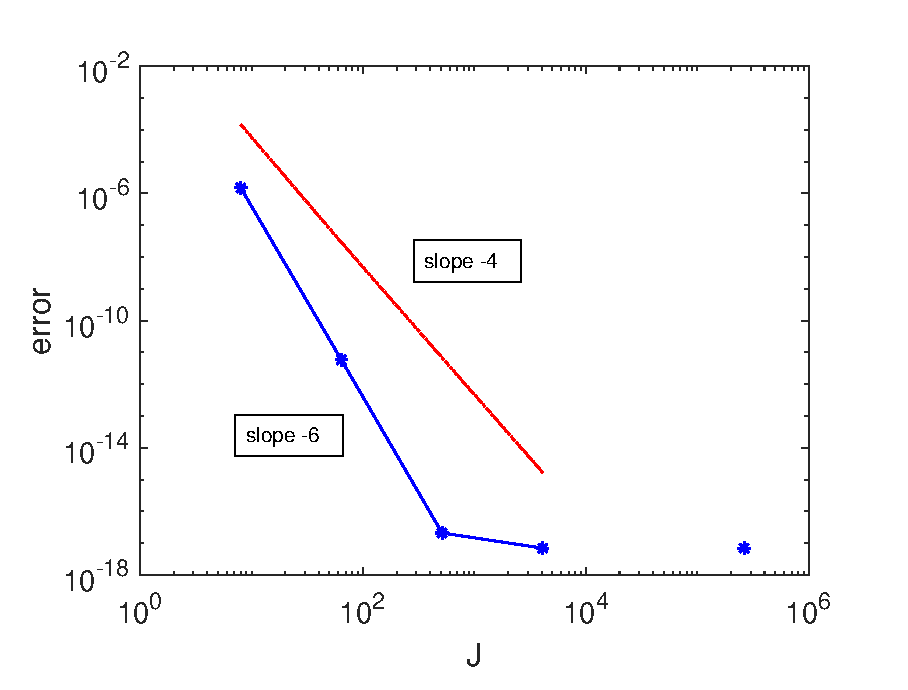
\includegraphics[width=0.45\linewidth]{Image1.eps}
  \hfill
  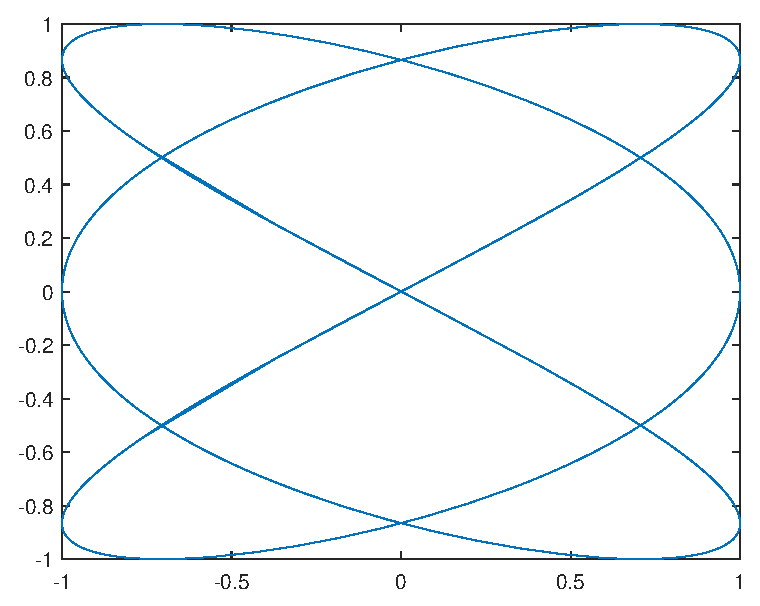
\includegraphics[width=0.45\linewidth]{Image2.eps}
  \caption{左: 图一的描述;~ 右:图二的描述.}
  \label{fig:image}
\end{figure}

通过 \verb|ref| 引用图片: 图 \ref{fig:data}.

通过 \verb|autoref| 引用图片: \autoref{fig:Image1} 与 \autoref{fig:Image2}.


使用 minipage 排版并排插图, 每个图都有单独的标题.

\begin{figure}[htp!]
\begin{minipage}[t]{0.48\linewidth}
\centering
  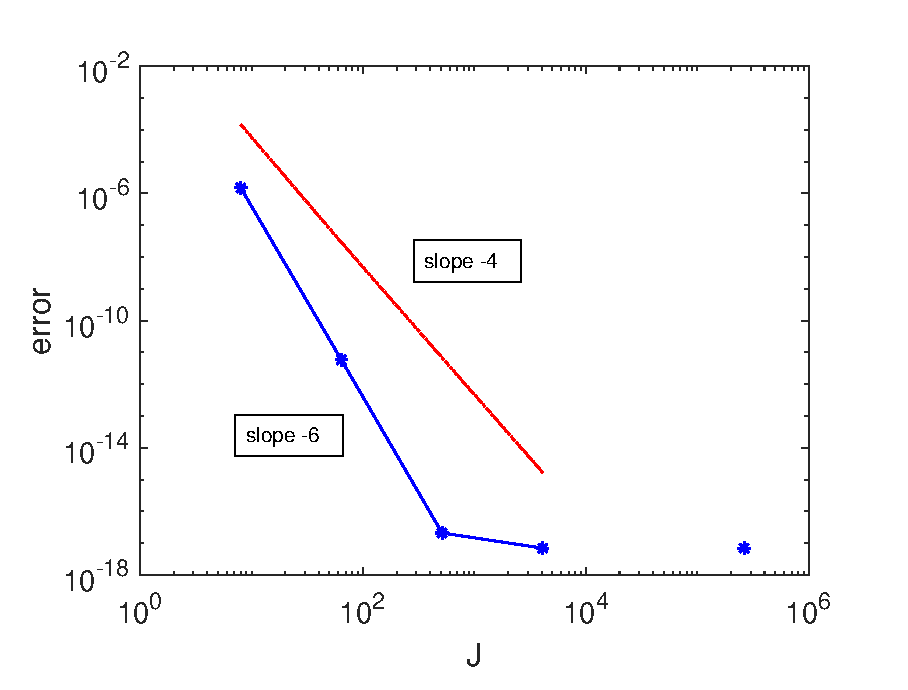
\includegraphics[width=0.9\linewidth]{Image1.eps}
    \caption{图一的描述.}
    \label{fig:Image1}
\end{minipage}
  \hfill
\begin{minipage}[t]{0.48\linewidth}
\centering
   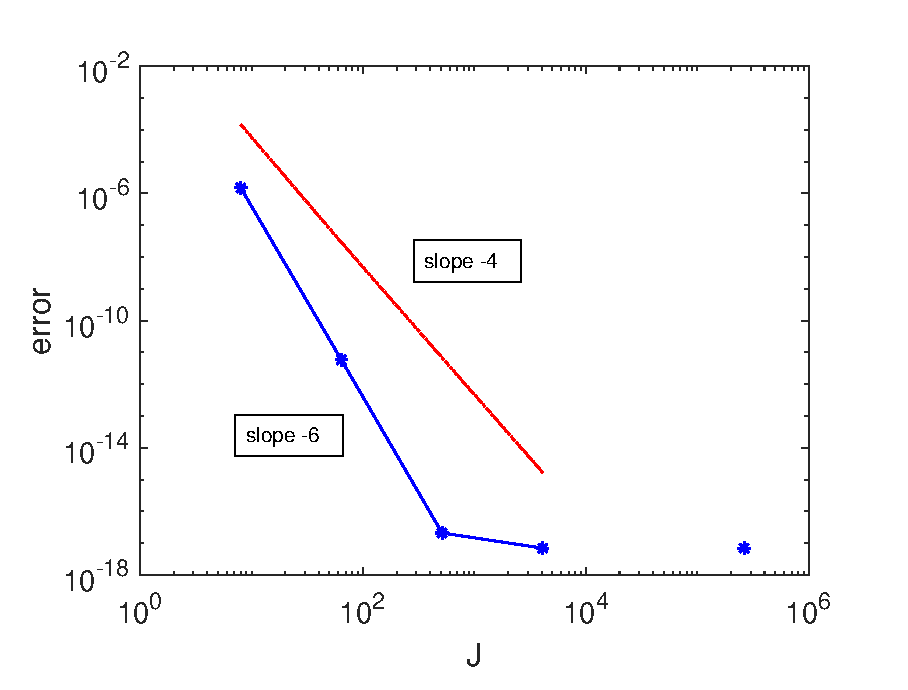
\includegraphics[width=0.9\linewidth]{Image1.eps}
   \caption{图二的描述.}
   \label{fig:Image2}
\end{minipage}
\end{figure}

使用 subfig 宏包实现多图并排.
\begin{figure}[htp!]
\centering
\subfloat[Subcaption A]{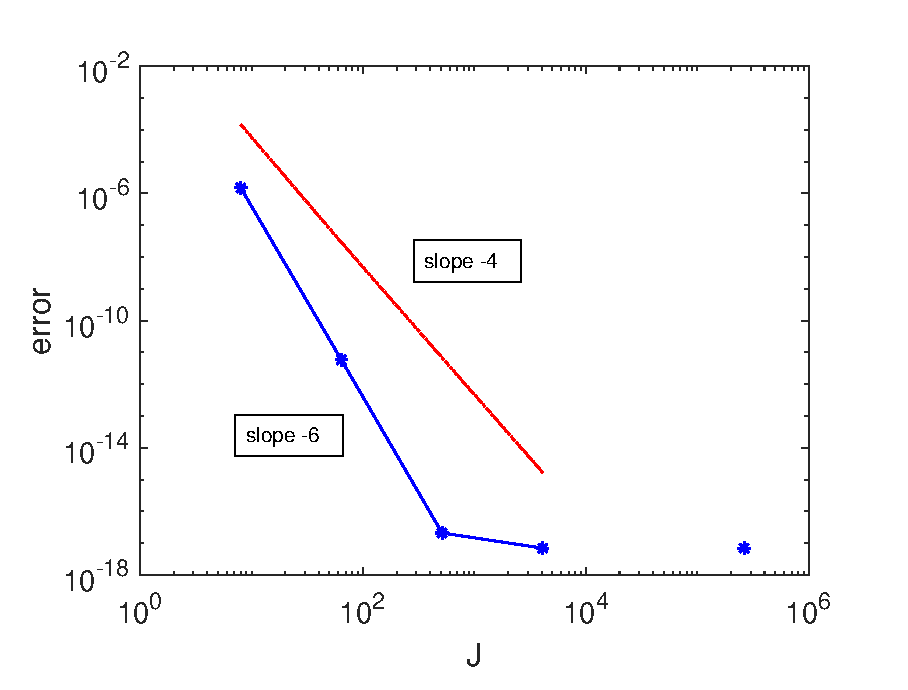
\includegraphics[width=0.3\linewidth]{Image1}}
\hfill
\subfloat[Subcaption B]{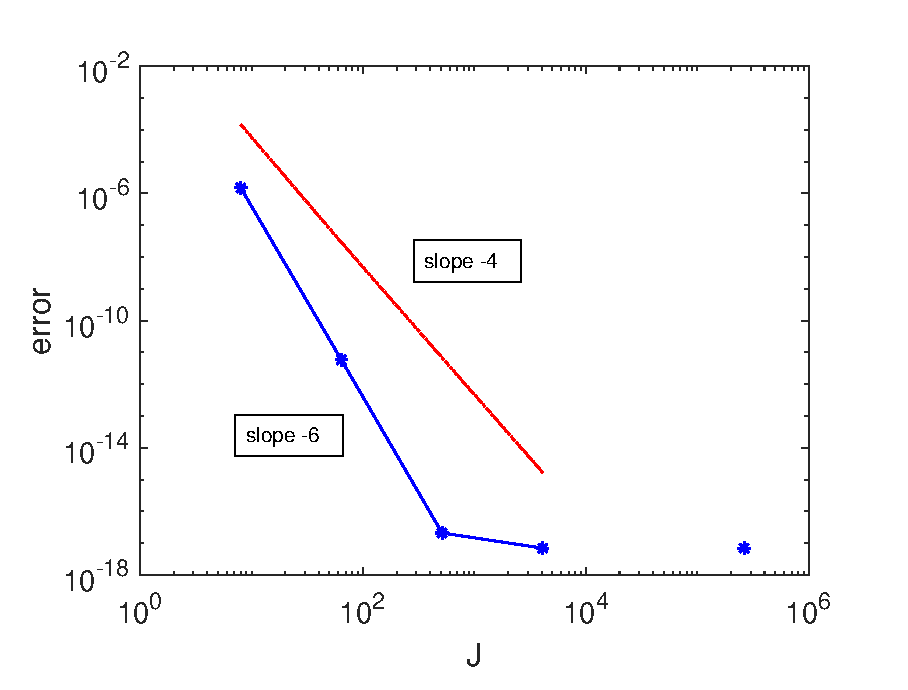
\includegraphics[width=0.3\linewidth]{Image1}}
\hfill
\subfloat[Subcaption C]{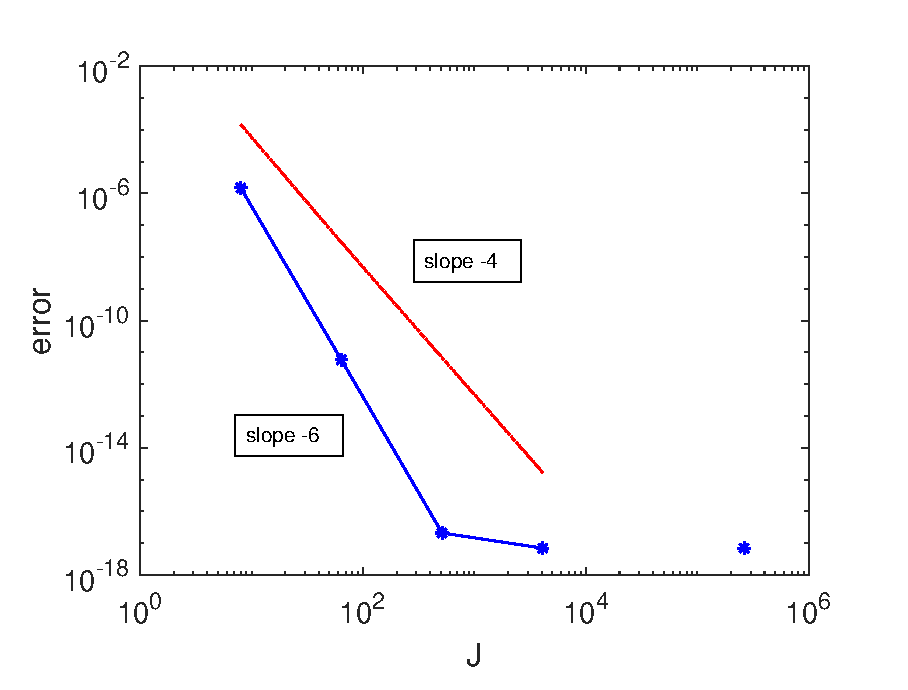
\includegraphics[width=0.3\linewidth]{Image1}} \\
\subfloat[Subcaption D]{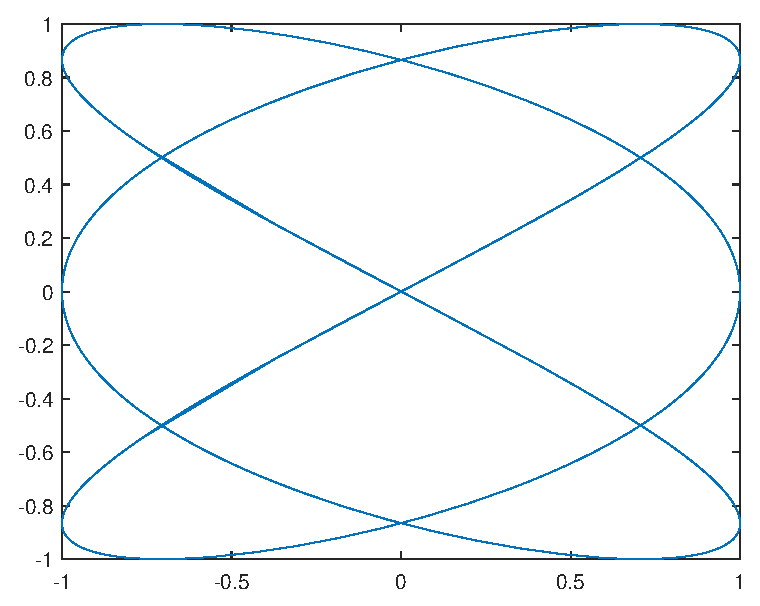
\includegraphics[width=0.3\linewidth]{Image2}}
\hfill
\subfloat[Subcaption E]{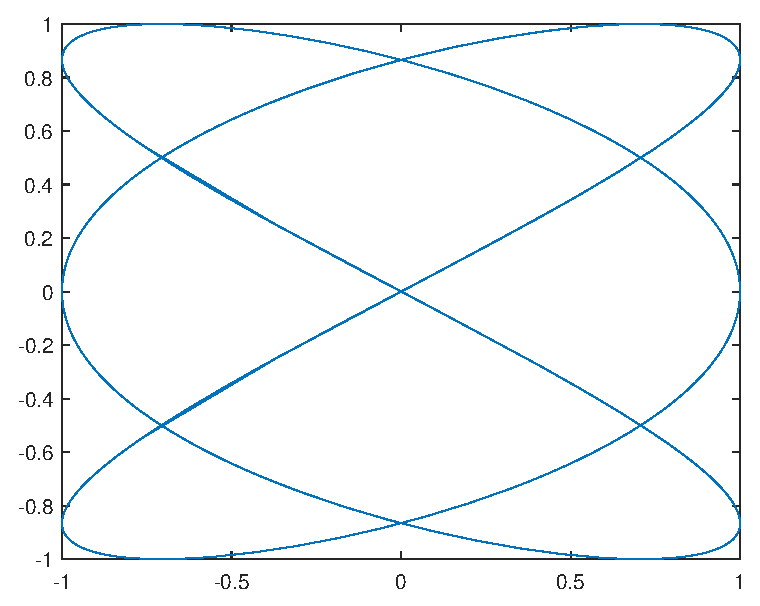
\includegraphics[width=0.3\linewidth]{Image2}}
\hfill
\subfloat[Subcaption F]{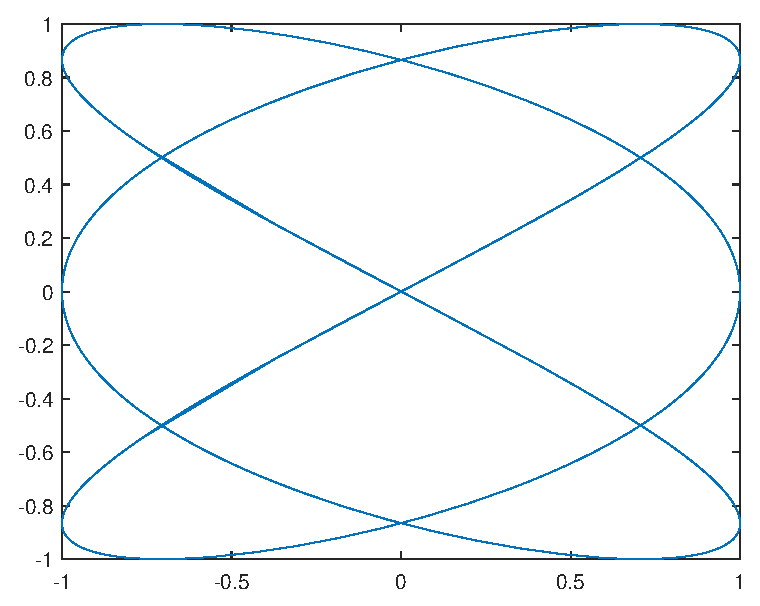
\includegraphics[width=0.3\linewidth]{Image2}}
\caption{六个图并排.}
\end{figure}



%%%%%%%%%%%%%%%%%%%%%%%%%%%% 列表与参考文献  %%%%%%%%%%%%%%%%%%%%%%%%%%%%%%%

\chapter{列表与参考文献}

\section{列表的使用}

这是一个计数的列表.
\begin{enumerate}
	\item 第一项
		\begin{enumerate}
			\item 第一项中的第一项
			\item 第一项中的第二项
		\end{enumerate}
	\item 第二项
	\item 第三项
\end{enumerate}


这是一个不计数的列表.
\begin{itemize}%[label={$\bullet$}]
	\item 第一项
	\begin{itemize}
		\item 第一项中的第一项
		\item 第一项中的第二项
	\end{itemize}
	\item 第二项
	\item 第三项
\end{itemize}


\section{参考文献}

参考文献采用 BibLaTeX 的方式生成 (内容写在文件 \verb|mybib.bib| 中), 参考文献的样式 \verb|shnuthesis-numeric| 参考了 清华大学 LaTeX 模板 \href{https://github.com/tuna/thuthesis}{\fbox{thuthesis}} 的文献样式, 去掉了文献的标号 [J], [M]等, 如果想要文献的标号可以选择  \verb|thuthesis-numeric| 格式. 参考文献的样式还可以选择 BibLaTeX 的标准样式: \verb|plain|、\verb|abbrv|、\verb|unsrt| 与 \verb|siam| 等.

文献引用 \cite{Adams2003, Tadmor2012}和 \cite{LiLiu1997}.


%%%%%%%%%%%%%%%%%%%%%%%%%%%%%%%%%%%%%%%%%%%%%%%%%%%%%%%%%%%%%%%%%%%%%%%%%%

\backmatter  % 结束章节自动编号

%%%%%%%%%%%%%%%%%%%%%%%% 生成参考文献  %%%%%%%%%%%%%%%%%%%%%%%%%%%%%%%%%%%%%

% 生成参考文献, 使用第二种请把第一种全部注释

% 第一种方式, 使用 bib 文件

%\nocite{*}  % 可以暂时显示全部参考文献, 包括未引用的

% 使用方法:\bibliography{参考文件1文件名, 参考文献2文件名, ...}
% 参考文献格式可选  plain, abbrv, unsrt, siam
% \bibliographystyle{plain}
% \bibliographystyle{thuthesis-numeric}
\bibliographystyle{shnuthesis-numeric}
\bibliography{mybib}


% 第二种方式, 按照格式直接写文献信息

%\begin{thebibliography}{99}
%
%\bibitem{Adams2003} Adams~R~A, Fournier~J~J~F. Sobolev spaces. Elsevier, 2003.
%
%\bibitem{Shen1994} Shen~J. Efficient spectral-Galerkin method I. Direct solvers of second- and fourth-order equations using Legendre polynomials. SIAM J. Sci. Comput., 1994, 15(6): 1489-1505.
%
%\bibitem{Tadmor2012} Tadmor~E. A review of numerical methods for nonlinear partial differential
%  equations. Bull. Amer. Math. Soc., 2012, 49(4): 507-554.
%
%\bibitem{TreWei2014}Trefethen~L~N, Weideman~J~A~C. The exponentially convergent trapezoidal rule. SIAM Rev., 2014, 56(3): 385-458.
%
%\bibitem{LiLiu1997} 李荣华, 刘播. 微分方程数值解法. 东南大学出版社, 1997.
%
%\end{thebibliography}



%%%%%%%%%%%%%%%%%%%%%% 攻读硕士学位期间的研究成果  %%%%%%%%%%%%%%%%%%%%%%%%%%%

\begin{researchpage}
\hangindent 1.4em
\noindent
[1] {{\bf Author 1} and Author 2},  The name of the published article 1, {\bf  Name of Journal}, 2020, 12(34):1001-1020.

\hangindent 1.4em
\noindent
[2] {{\bf Author 1},  Author 2 and Author 3}, The name of the published article 2, submitted to
Journal of XXX.


\end{researchpage}



%%%%%%%%%%%%%%%%%%%%%%%%%%% Thanks page %%%%%%%%%%%%%%%%%%%%%%%%%%%%%%%%%%%%

\begin{thankpage}
\chaptermark{致谢}
\setlength{\baselineskip}{24pt}

感谢老师感谢老师感谢老师感谢老师感谢老师感谢老师感谢老师感谢老师感谢老师感谢老师感谢老师感谢老师感谢老师感谢老师感谢老师感谢老师感谢老师感谢老师感谢老师感谢老师感谢老师感谢老师感谢老师感谢老师感谢老师感谢老师感谢老师感谢老师感谢老师感谢老师感谢老师感谢老师感谢老师感谢老师感谢老师感谢老师.

感谢老师感谢老师感谢老师感谢老师感谢老师感谢老师感谢老师感谢老师感谢老师感谢老师感谢老师感谢老师感谢老师感谢老师感谢老师感谢老师感谢老师感谢老师感谢老师感谢老师感谢老师感谢老师感谢老师感谢老师感谢老师感谢老师.

感谢老师感谢老师感谢老师感谢老师感谢老师感谢老师感谢老师感谢老师感谢老师感谢老师感谢老师感谢老师感谢老师感谢老师感谢老师感谢老师感谢老师感谢老师感谢老师感谢老师感谢老师感谢老师感谢老师感谢老师感谢老师感谢老师感谢老师感谢老师感谢老师感谢老师感谢老师感谢老师感谢老师感谢老师感谢老师感谢老师.


\end{thankpage}


%%%%%%%%%%%%%%%%%%%%%%%% 附录  %%%%%%%%%%%%%%%%%%%%%%%%%%%%%%%%%%%%%%%

% 添加附录, 如不需要可以注释掉
\appendix

%\setcounter{page}{1} % 如果需要可以自行重置页码
\renewcommand{\chaptermark}[1]{\markboth{#1}{}}
\chapter{附录 A ~ 这是第一个附录}
\renewcommand{\thesection}{A.\arabic{section}}
\section{附录A的小节}

这里是附录环境, 手动设置了 chapter 和 section 的样式, 并且加入到了目录.

\chapter{附录 B ~ 这是第二个附录}
\renewcommand{\thesection}{B.\arabic{section}}
\section{附录B的小节}

这里是附录环境, 手动设置了 chapter 和 section 的样式, 并且加入到了目录.



\end{document}



